\documentclass[conference]{IEEEtran}
\IEEEoverridecommandlockouts

\usepackage{cite}
\usepackage{amsmath,amssymb,amsfonts}
\usepackage{amsbsy}
\usepackage{mathtools}
\usepackage{algorithmic}
\usepackage{graphicx}
\usepackage{textcomp}
\usepackage{xcolor}
\usepackage{textcomp}
\usepackage{float}
\usepackage{array}
\usepackage{siunitx}
\usepackage{tabularx}
\usepackage{listings}
\usepackage{accents}
\usepackage{nicematrix,tikz}
\usepackage{setspace}
\usepackage[colorlinks=false]{hyperref}
\def\BibTeX{{\rm B\kern-.05em{\sc i\kern-.025em b}\kern-.08em
    T\kern-.1667em\lower.7ex\hbox{E}\kern-.125emX}}

\setlength{\parindent}{0pt}

% Define the custom column type Y
\newcolumntype{Y}{>{\centering\arraybackslash} m{0.9cm}}

\definecolor{codeblue}{rgb}{0.2,0.2,0.6}
\definecolor{codegreen}{rgb}{0.133,0.545,0.133}
\definecolor{codegray}{rgb}{0.5,0.5,0.5}
\definecolor{codepurple}{rgb}{0.58,0,0.82}
\definecolor{backcolour}{rgb}{0.95,0.95,0.92}

\lstdefinestyle{mystyle}{
    backgroundcolor=\color{backcolour},
    commentstyle=\color{codegreen},
    keywordstyle=\color{codeblue},
    numberstyle=\tiny\color{codegray},
    stringstyle=\color{codepurple},
    basicstyle=\ttfamily\scriptsize,
    breakatwhitespace=false,
    breaklines=true,
    captionpos=b,
    keepspaces=true,
    numbers=none,
    numbersep=5pt,
    showspaces=false,
    showstringspaces=false,
    showtabs=false,
    tabsize=2
}
\lstset{style=mystyle}

\title{Robotics and Mechatronics\\
{\LARGE Homework Four}
}

\author{\IEEEauthorblockN{Mohammad Montazeri}
    \IEEEauthorblockA{\textit{School of Mechanical Engineering} \\
        \textit{College of Engineering, University of Tehran}\\
        Tehran, Iran; 810699269 \\
        mohammadmontazeri@ut.ac.ir}
}

\begin{document}
\maketitle

\begin{abstract}
    This assignment explores serial manipulator dynamics in robotics, covering inverse dynamics (IDP), forward dynamics (FDP), inverse kinematics (IKP), and forward kinematics (FKP). By applying Newtonian and Lagrangian methods, we derive essential equations and concentrate on them.
\end{abstract}

\begin{IEEEkeywords}
    Dynamics, Newtonian, Lagrangian, kinematics, velocity, acceleration, force
\end{IEEEkeywords}

\section{Introduction}
Robotic manipulators are integral to modern industries, from manufacturing to healthcare. In this assignment, we delve into the intricacies of IDP, FDP, IKP, and FKP. These concepts form the foundation for efficient robot control and design, enabling precise movements and task execution.

\section{Problem 1: IKP}
\textbf{FKP Equations}: Having $\theta_1$, $\theta_2$ and $\theta_3$, we want to find $x, y$ and $\phi$ of end-effector.
\begin{align}
    x =    & L_1 \cos (\theta_1) + L_2 \cos (\theta_1 + \theta_2) + L_3 \cos (\theta_1 + \theta_2 + \theta_3) \\
    y =    & L_1 \sin (\theta_1) + L_2 \sin (\theta_1 + \theta_2) + L_3 \sin (\theta_1 + \theta_2 + \theta_3) \\
    \phi = & \theta_1 + \theta_2 + \theta_3
\end{align}

we're given:
\begin{footnotesize}
    \begin{align*}
        x =    & L_1  \cos\left(\frac{\pi}{4} + \frac{\pi}{9} \sin\left(\frac{\pi}{5} t\right) \right) + L_2 \cos\left(\frac{5\pi}{12} + \frac{\pi}{9} \sin\left(\frac{\pi}{5} t\right) + \frac{\pi}{18} \cos\left(\frac{\pi}{10} t\right)\right) + \\
               & L_3 \cos\left(\frac{11\pi}{36} + \frac{\pi}{9} \sin\left(\frac{\pi}{5} t\right) + \frac{\pi}{18} \cos\left(\frac{\pi}{10} t\right) - \frac{\pi}{36} \sin\left(\frac{\pi}{15} t\right) \right)                                      \\
        y =    & L_1  \sin\left(\frac{\pi}{4} + \frac{\pi}{9} \sin\left(\frac{\pi}{5} t\right) \right) + L_2 \sin\left(\frac{5\pi}{12} + \frac{\pi}{9} \sin\left(\frac{\pi}{5} t\right) + \frac{\pi}{18} \cos\left(\frac{\pi}{10} t\right)\right) + \\
               & L_3 \sin\left(\frac{11\pi}{36} + \frac{\pi}{9} \sin\left(\frac{\pi}{5} t\right) + \frac{\pi}{18} \cos\left(\frac{\pi}{10} t\right) - \frac{\pi}{36} \sin\left(\frac{\pi}{15} t\right) \right)                                      \\
        \phi = & \frac{\pi}{4} + \frac{\pi}{9} \sin\left(\frac{\pi}{5} t\right) + \frac{\pi}{6} + \frac{\pi}{18} \cos\left(\frac{\pi}{10} t\right) - \frac{\pi}{9} - \frac{\pi}{36} \sin\left(\frac{\pi}{15} t\right)
    \end{align*}
\end{footnotesize}

comparing the given equations and the derived ones gives:
\begin{align}
     & \theta_1 = \frac{\pi}{4} + \frac{\pi}{9} \sin\left(\frac{\pi}{5} t\right)     \\
     & \theta_2 = \frac{\pi}{6} + \frac{\pi}{18} \cos\left(\frac{\pi}{10} t\right)   \\
     & \theta_3 = - \frac{\pi}{9} - \frac{\pi}{36} \sin\left(\frac{\pi}{15} t\right)
\end{align}

\textbf{IKP Equations}: Assuming desired value(s) for $t$ and substituting in the given equations for $x, y \,\text{and}\, \phi$, we can find the task-space parameters. Having $x, y$ and $\phi$ of end-effector, we want to find $\theta_1$, $\theta_2$ and $\theta_3$ using IKP equations.
\begin{align*}
     & x            = L_1 \cos \theta_1 + L_2 \cos (\theta_1 + \theta_2) + L_3 \cos \phi                         \\
     & y            = L_1 \sin \theta_1 + L_2 \sin (\theta_1 + \theta_2) + L_3 \sin \phi                         \\
     & \rightarrow (x - L_1 \cos \theta_1 - L_3 \cos \phi)^2 + (y - L_1 \sin \theta_1 - L_3 \sin \phi)^2 = L_2^2
\end{align*}

\begin{gather}
    A \cos \theta_1 + B \sin \theta_1 = C \label{eq:IKP} \\
    A = 2 L_1 (x - L_3 \cos \phi)         \\
    B = 2 L_1 (y - L_3 \sin \phi)         \\
    C = x^2 + y^2 + L_1^2 - L_2^2 + L_3^2 - 2 L_3 (x \cos \phi + y \sin \phi)
\end{gather}

\begin{large}
    \begin{align*}
         & Answers \longrightarrow
        \begin{cases}
            \theta_1 ^+ \longrightarrow\theta_2 ^+ \longrightarrow \theta_3 ^+ \\[20pt]
            \theta_1 ^- \longrightarrow\theta_2 ^- \longrightarrow \theta_3 ^-
        \end{cases}
    \end{align*}
\end{large}

We use MATLAB to iteratively calculate the output of both methods for a desired range of $t=[0, 10](s)$ with a step size of $\Delta t = 0.1(s)$ resulting in 101 samples. The MATLAB code is attached to this report, while here are its results:
\begin{figure}[htbp]
    \centerline{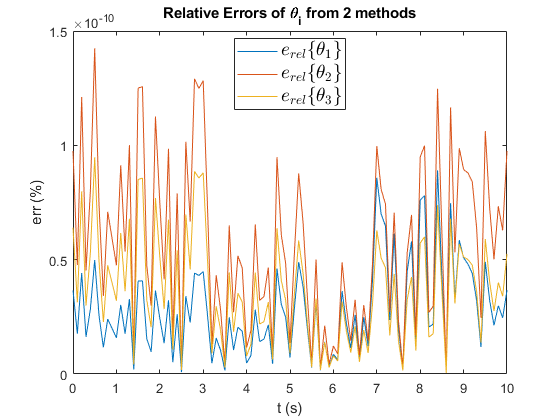
\includegraphics[width=0.4\textwidth]{figures/prob1a.png}}
    \caption{The differences between joint space angles computed directly and from IKP equations.}
    \label{fig:res1}
\end{figure}

\begin{figure}[htbp]
    \centerline{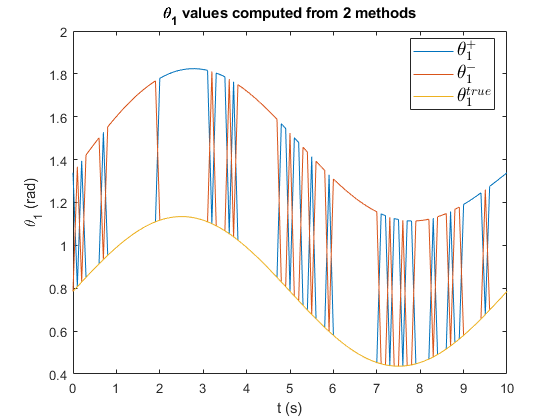
\includegraphics[width=0.4\textwidth]{figures/prob1b.png}}
    \caption{$\theta_1$ angles computed directly or from IKP}
    \label{fig:res2}
\end{figure}

\begin{figure}[htbp]
    \centerline{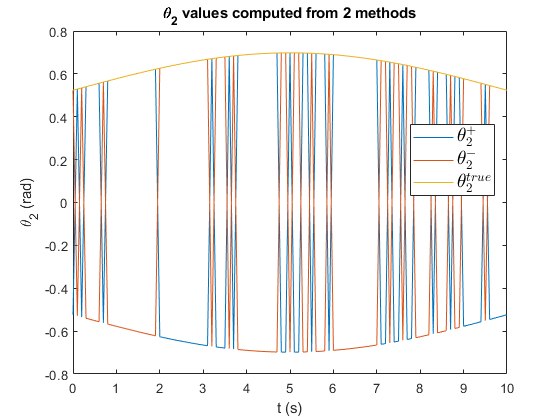
\includegraphics[width=0.4\textwidth]{figures/prob1c.png}}
    \caption{$\theta_2$ angles computed directly or from IKP}
    \label{fig:res3}
\end{figure}

\begin{figure}[H]
    \centerline{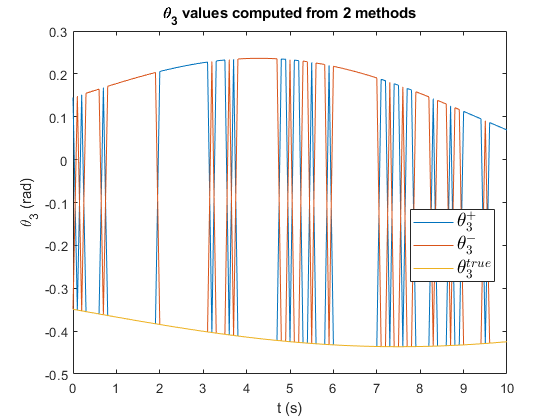
\includegraphics[width=0.4\textwidth]{figures/prob1d.png}}
    \caption{$\theta_3$ angles computed directly or from IKP}
    \label{fig:res4}
\end{figure}

It's worth mentioning that solving via IKP gives two values for each of $\theta_i$, while one of them is the desired one. By eliminating the answer which is further from the actual one computed directly, the following result will be achieved:

\begin{figure}[H]
    \centerline{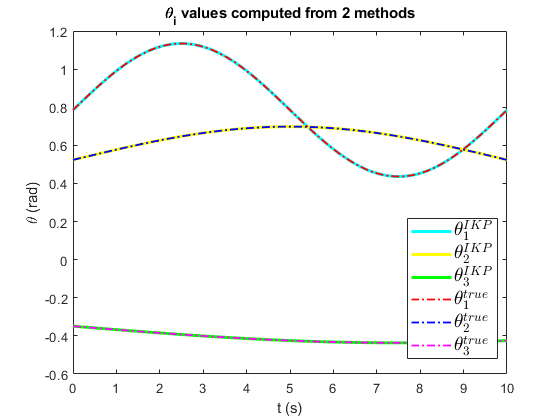
\includegraphics[width=0.4\textwidth]{figures/prob1e.png}}
    \caption{summary of final $\theta_i$ angles computed directly or from IKP}
    \label{fig:res5}
\end{figure}

As it can be seen, the duality of answers for each angle found in Figures~\ref{fig:res2} to \ref{fig:res4} has vanished in Figure~\ref{fig:res5}. It's also seen that both methods predict the same angles and have a quite nice conformity. It must also be noted that Figure~\ref{fig:res1} shows the relative error between the results of both direct and IKP methods, where the answer chose as the result of IKP method is the one shown in Figure~\ref{fig:res5}, meaning the closest answer to the expected one. Thus, it's seen that the errors are all quite low, in an order of $10^{-10}$.
\vspace{10px}

\section{Problem 2: A Walk in the Park}
\begin{gather}
    \dot{\vec{P}} = \, \left]\dot{\vec{P}}\right[ \, + \vec{\omega}\times\vec{P} \\
        \ddot{\vec{P}} = \, \left]\ddot{\vec{P}}\right[ \, + \vec{\omega}\times\dot{\vec{P}}
\end{gather}

\begin{align*}
    \vec{\omega}(t) & = t \hat{\imath} - t^2 \hat{\jmath} + \frac{1}{t+1} \hat{k} \\
    \vec{P}(t)      & = 2t^2 \hat{\imath}^\prime + t \hat{\jmath}^\prime          \\
\end{align*}

\begin{figure}[htbp]
    \centerline{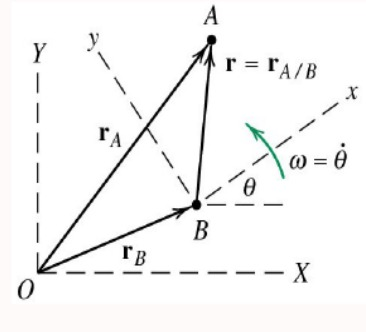
\includegraphics[width=0.35\textwidth]{figures/prob2a.jpeg}}
    \caption{Motion Relative to Rotating Axex \cite{b4}}
    \label{fig:prob2a}
\end{figure}

\begin{align*}
    ]\dot{\vec{P}}[  & = 4t \hat{\imath}^\prime + \hat{\jmath}^\prime                                                                                                                                \\
    \dot{\vec{P}}    & = (4t \hat{\imath}^\prime + \hat{\jmath}^\prime) + (t \hat{\imath} - t^2 \hat{\jmath} + \frac{1}{t+1} \hat{k})\times(2t^2 \hat{\imath}^\prime + t \hat{\jmath}^\prime)        \\
                     & = \begin{bmatrix}
                                 4t \\
                                 1  \\
                                 0
                             \end{bmatrix} + \begin{bmatrix}
                                                 t    \\
                                                 -t^2 \\
                                                 \frac{1}{t+1}
                                             \end{bmatrix} \times \begin{bmatrix}
                                                                      2t^2 \\
                                                                      t    \\
                                                                      0
                                                                  \end{bmatrix} = \left(\begin{array}{c} 4\,t-\frac{t}{t+1} \\[10px]
                                                                                                \frac{2\,t^2}{t+1}+1   \\[10px]
                                                                                                2\,t^4+t^2\end{array}\right)                                                                      \\
    ]\ddot{\vec{P}}[ & = \frac{d(\dot{\vec{P}})}{dt} = (4-\frac{1}{(t+1)^2})\hat{\imath}^\prime + (\frac{2\,t\,\left(t+2\right)}{{\left(t+1\right)}^2})\hat{\jmath}^\prime + (8t^3+2t)\hat{k}^\prime \\
    \ddot{\vec{P}}   & =  \begin{bmatrix}
                              4-\frac{1}{(t+1)^2}                                 \\[10px]
                              \frac{2\,t\,\left(t+2\right)}{{\left(t+1\right)}^2} \\[10px]
                              8t^3+2t
                          \end{bmatrix} + \begin{bmatrix}
                                              t    \\[10px]
                                              -t^2 \\[10px]
                                              \frac{1}{t+1}
                                          \end{bmatrix} \times \begin{bmatrix}
                                                                   4\,t-\frac{t}{t+1}   \\[10px]
                                                                   \frac{2\,t^2}{t+1}+1 \\[10px]
                                                                   2\,t^4+t^2
                                                               \end{bmatrix}                                                                                     \\
                     & = \left(\begin{array}{c} \frac{4\,t^2+8\,t+3}{{\left(t+1\right)}^2}-t^2\,\left(2\,t^4+t^2\right)-\frac{\frac{2\,t^2}{t+1}+1}{t+1}  \\[10px]
                                       \frac{4\,t-\frac{t}{t+1}}{t+1}-t\,\left(2\,t^4+t^2\right)+\frac{2\,t\,\left(t+2\right)}{{\left(t+1\right)}^2} \\[10px]
                                       2\,t+t^2\,\left(4\,t-\frac{t}{t+1}\right)+t\,\left(\frac{2\,t^2}{t+1}+1\right)+8\,t^3\end{array}\right)
\end{align*}

Deriving the dynamic equations according to Figure~\ref{fig:prob2a} gives \cite{b5}:
\begin{gather}
    \vec{V}_A = \vec{V}_B + \vec{\omega} \times \vec{r}_{B/A} + \vec{V}_{rel} \label{eq:Vrel}
\end{gather}

\begin{figure}[htbp]
    \centerline{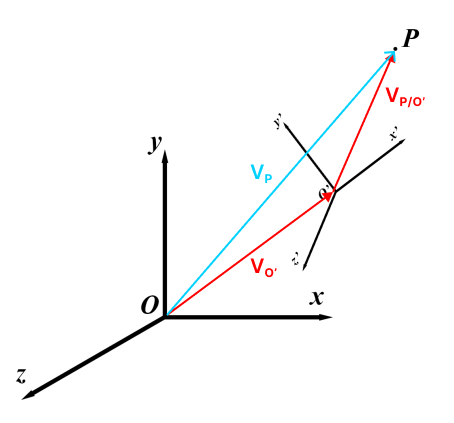
\includegraphics[width=0.4\textwidth]{figures/prob2b.png}}
    \caption{Dynamics of problem under review}
    \label{fig:prob2b}
\end{figure}

In this problem, with a glance of Figure~\ref{fig:prob2b} and comparing it with Figure~\ref{fig:prob2a}, we can modify equation \ref{eq:Vrel} as:
\begin{gather}
    \mathbf{V}_P = \mathbf{V}_{O^\prime} + \mathbf{V}_{P/O^\prime} \\
    \mathbf{a}_P = \mathbf{a}_{O^\prime} + \mathbf{a}_{P/O^\prime}
\end{gather}

where,

\begin{align*}
    \vec{O^\prime}(t)     & = (1+t) \hat{\imath} + t \hat{\jmath} + t \hat{k} \longrightarrow \\
    \mathbf{V}_{O^\prime} & = \dot{\vec{O^\prime}}(t) = \hat{\imath} + \hat{\jmath} + \hat{k} \\
    \mathbf{a}_{O^\prime} & = \dot{\vec{V}}_{O^\prime}(t) = \vec{0}
\end{align*}

so,
\begin{gather}
    \mathbf{V}_P = \begin{bmatrix}
        1 \\
        1 \\
        1
    \end{bmatrix} + \begin{bmatrix}
        4\,t-\frac{t}{t+1} \\ \frac{2\,t^2}{t+1}+1\\ 2\,t^4+t^2
    \end{bmatrix} = \begin{bmatrix}
        \frac{{\left(2\,t+1\right)}^2}{t+1} \\[10px]
        \frac{2\,t^2}{t+1}+2                \\[10px]
        2\,t^4+t^2+1
    \end{bmatrix}                                                                                          \\[5px]
    \mathbf{a}_P = \vec{0} + \ddot{\vec{P}} = \begin{bmatrix}
        -\frac{2\,t^8+4\,t^7+3\,t^6+2\,t^5+t^4-2\,t^2-7\,t-2}{{\left(t+1\right)}^2}          \\[10px]
        -\frac{t\,\left(2\,t^6+4\,t^5+3\,t^4+2\,t^3+t^2-6\,t-7\right)}{{\left(t+1\right)}^2} \\[10px]
        \frac{t\,\left(12\,t^3+13\,t^2+3\,t+3\right)}{t+1}
    \end{bmatrix}
\end{gather}


% \begin{gather}
%     \mathbf{V}_P = \mathbf{V}_{O^\prime} + \vec{\omega} \times \mathbf{r}_{P/O^\prime} + \mathbf{V}_{P/O^\prime}
% \end{gather}

% where we're given with:
% \begin{align*}
%     \vec{O^\prime}(t)       & = (1+t) \hat{\imath} + t \hat{\jmath} + t \hat{k}                                              \\
%     \vec{\omega}(t)         & = t \hat{\imath} - t^2 \hat{\jmath} + \frac{1}{t+1} \hat{k}                                    \\
%     \vec{P}(t)              & = 2t^2 \hat{\imath}^\prime + t \hat{\jmath}^\prime                                             \\
%     \mathbf{V}_{O^\prime}   & = \dot{\vec{O^\prime}}(t) = \hat{\imath} + \hat{\jmath} + \hat{k}                              \\
%     \mathbf{r}_{P/O^\prime} & = \vec{P} = 2t^2 \hat{\imath}^\prime + t \hat{\jmath}^\prime                                   \\
%     \mathbf{V}_{P/O^\prime} & = \dot{\mathbf{r}}_{P/O^\prime} = \dot{\vec{P}} = 4t \hat{\imath}^\prime + \hat{\jmath}^\prime \\
%     % \dot{\vec{P}} &= (4t \hat{\imath}^\prime + \hat{\jmath}^\prime) + (t \hat{\imath} - t^2 \hat{\jmath} + \frac{1}{t+1} \hat{k})\times(2t^2 \hat{\imath}^\prime + t \hat{\jmath}^\prime) \\
%     % ]\ddot{\vec{P}}[ &= 4 \hat{\imath}^\prime
% \end{align*}
% \begin{align*}
%     \mathbf{V}_P = (\hat{\imath} + \hat{\jmath} + \hat{k}) + (t \hat{\imath} - t^2 \hat{\jmath} + \frac{1}{t+1} \hat{k}) \times (2t^2 \hat{\imath}^\prime + t \hat{\jmath}^\prime) + (4t \hat{\imath}^\prime + \hat{\jmath}^\prime)
% \end{align*}

\vspace{35px}

\section{Problem 3: Isaac vs Joseph}
Assuming massless rods in pendulums, their \textit{Inertia} is equal to $I = m_p l^2$ where $m_p$ is the mass of the pendulum and $l$ is the length of its connecting rod.
Now we can derive the \textbf{Newton} equilibrium after sketching FBD for each element of the system. Note that it's assumed that the free length\footnote{Initial length of the spring where it doesn't apply any force; in this case, the length of the spring when it has fully vertical orientation, resulting in $x_1 = x_2 = 0$.} of the spring is equal to $l$. The positive direction of x-axis is also assumed to be horizontally rightwards and the y-axis, vertically upwards. The carts don't have vertical displacement either.
\subsection{Newtonian Approach}
\begin{figure}[htbp]
    \centerline{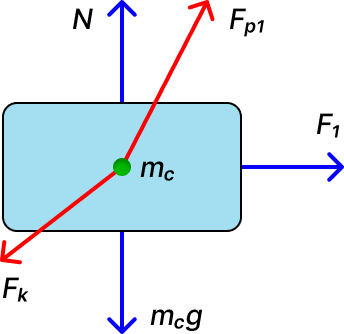
\includegraphics[width=0.3\textwidth]{figures/cart1.png}}
    \caption{Free Body Diagram of upper cart}
    \label{fig:cart1}
\end{figure}

% \begin{equation}
\begin{align}
     & \sum F_x=m a_x \rightarrow F_1 + F_{p_1} \sin \theta_1 - F_k \cos \alpha = m_c \ddot{x}_1     \nonumber            \\
     & \sum F_y=m a_y \rightarrow N_1 + F_{p_1} \left|\cos \theta_1\right| - F_k \sin \alpha - m_c g = 0 \nonumber        \\
     & \alpha = \arctan \left(\frac{l}{x_1+x_2}\right) \quad (\text{\small the angle spring makes with x-axis}) \nonumber \\
     & F_k = k \Delta l = k \left(\sqrt{\left(x_1+x_2\right)^2+l^2}-l\right) \label{eq:newton1}
\end{align}
% \end{equation}

\begin{figure}[htbp]
    \centerline{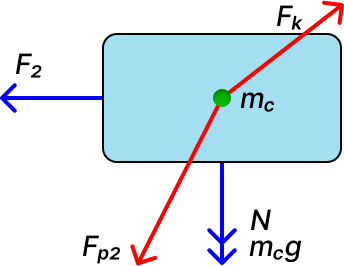
\includegraphics[width=0.3\textwidth]{figures/cart2.png}}
    \caption{Free Body Diagram of lower cart}
    \label{fig:cart2}
\end{figure}

\begin{equation}
    \begin{aligned}
         & \sum F_x=m a_x \rightarrow -F_2 - F_{p_2} \sin \theta_2 + F_k \cos \alpha = m_c \ddot{x}_2         \\
         & \sum F_y=m a_y \rightarrow -N_2 - F_{p_2} \left|\cos \theta_2\right| + F_k \sin \alpha - m_c g = 0
    \end{aligned}
\end{equation}

\begin{figure}[htbp]
    \centerline{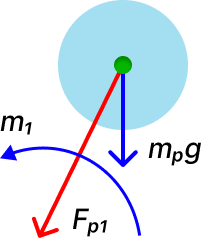
\includegraphics[width=0.2\textwidth]{figures/pendulum1.png}}
    \caption{Free Body Diagram of upper pendulum}
    \label{fig:pen1}
\end{figure}

Writing the equilibrium of momentum for pendulums is a little bit tricky. In the following equations, a second term is added to the right hand side of the equation which might seem confusing. That's because these equations are NOT written about the centre of mass; rather, they're about the point where the connecting rod is attached to the carts, at their center point. Thus, a \textit{Torque of CoM} also appears in the RHS.
\begin{align}
     & \sum M_A=I_A \ddot{\theta}_1+m_p \bar{a} d \Longrightarrow \nonumber                                               \\
     & M_1-m_p g l \sin \theta_1=m_p l^2 \ddot{\theta}_1+m_p\left(l^2 \ddot{\theta}_1-\ddot{x}_1 l \cos \theta_1\right)   \\
     & \sum F_x = m a_x \Longrightarrow \nonumber                                                                         \\
     & -F_{p_1} \sin \theta_1=m_p\left(\ddot{x}_1+l \dot{\theta}_1^2 \sin \theta_1-l \ddot{\theta}_1 \cos \theta_1\right)
\end{align}

\begin{figure}[htbp]
    \centerline{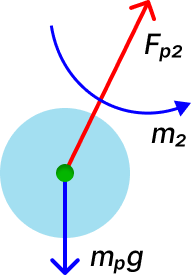
\includegraphics[width=0.2\textwidth]{figures/pendulum2.png}}
    \caption{Free Body Diagram of lower pendulum}
    \label{fig:pen2}
\end{figure}

\begin{align}
     & \sum M_B=I_B \ddot{\theta}_2+m_p \bar{a} d \Longrightarrow \nonumber                                                                 \\
     & M_2+m_p g l \sin \theta_2=m_p l^2 \ddot{\theta}_2+m_p\left(l^2 \ddot{\theta}_2-\ddot{x}_2 l \cos \theta_2\right)                     \\
     & \sum F_x = m a_x \Longrightarrow \nonumber                                                                                           \\
     & F_{p_2} \sin \theta_2=m_p\left(\ddot{x}_2+l \dot{\theta}_2^2 \sin \theta_2-l \ddot{\theta}_2 \cos \theta_2\right) \label{eq:newton6}
\end{align}

\vspace{20px}
Combining equations \ref{eq:newton1} to \ref{eq:newton6} gives
\begin{normalsize}
    \begin{equation}
        \begin{aligned}
            M_1 = & \, 2m_p l^2 \ddot{\theta}_1 - m_p l \ddot{x}_1 \cos \left(\theta_1\right) +m_p g l \sin \left(\theta_1\right) \\
            M_2 = & \, 2m_p l^2 \ddot{\theta}_2 - m_p l \ddot{x}_2 \cos \left(\theta_2\right) -m_p g l \sin \left(\theta_2\right) \\
            F_1 = & +k\left(\sqrt{\left(x_1+x_2\right)^2+l^2}-l\right) \cos \left(\tan ^{-1}\left(\frac{l}{x_1+x_2}\right)\right) \\
                  & -m_p\left(\ddot{x}_1+l \dot{\theta}_1^2 \sin \theta_1-l \ddot{\theta}_1 \cos \theta_1\right)+m_c \ddot{x}_1   \\
            F_2 = & -k\left(\sqrt{\left(x_1+x_2\right)^2+l^2}-l\right) \cos \left(\tan ^{-1}\left(\frac{l}{x_1+x_2}\right)\right) \\
                  & +m_p\left(\ddot{x}_2+l \dot{\theta}_2^2 \sin \theta_2-l \ddot{\theta}_2 \cos \theta_2\right)-m_c \ddot{x}_2
        \end{aligned}
    \end{equation}
\end{normalsize}

\subsection{Lagrangian Approach}
\begin{align*}
    T=           & \sum_{1}^{2}\frac{1}{2}m_c \dot{x}_i + \sum_{1}^{2}\frac{1}{2}m_p v_{p_i} = \frac{1}{2} m_c\left(\dot{x}_1^2+\dot{x}_2^2\right) +\frac{1}{2} m_p \times                                        \\
                 & \left(\dot{x}_1^2+\dot{x}_2^2+l^2\left(\dot{\theta}_1^2+\dot{\theta}_2^2\right)-2 l\left(\dot{x}_2 \dot{\theta}_2 \cos \theta_2+\dot{x}_1 \dot{\theta}_1 \cos \theta_1\right)\right)           \\
    V=           & \, U_k + U_g \footnotemark = \frac{1}{2} k {\Delta l}^2 + \sum_{1}^{2} m_p g h_i =                                                                                                             \\
                 & \frac{1}{2} k\left(\sqrt{\left(x_1+x_2\right)^2+l^2}-l\right)^2 + m g l \left(\cos \theta_2 - \cos \theta_1\right)                                                                             \\
    \mathcal{L}= & \, T-V \hspace{20px} \frac{d}{d t} \left(\frac{\partial \mathcal{L}}{\partial \dot{q}_i}\right)-\frac{\partial \mathcal{L}}{\partial q_i}=Q_i \hspace{20px} q_i = x_1, x_2, \theta_1, \theta_2
\end{align*}

\vspace{5px}
Now differentiating gives:

% Switch to single-column mode
\twocolumn[
    \begin{center}
            \setstretch{3} % Change the multiplier to control the line height
            \begin{align}
                 & {\scriptstyle q_1 = x_1, Q_1 = F_1} \rightarrow
                 & m_c \ddot{x}_1+m_p\left(\ddot{x}_1+l\left(\dot{\theta}_1^2 \sin \theta_1-\ddot{\theta}_1 \cos \theta_1\right)\right)-k\frac{\left(x_1+x_2\right)\left(\sqrt{\left(x_1+x_2\right)^2+l^2}-l\right)}{\sqrt{\left(x_1+x_2\right)^2+l^2}}=F_1 \\
                 & {\scriptstyle q_2 = x_2, Q_2 = F_2} \rightarrow
                 & m_c \ddot{x}_2+m_p\left(\ddot{x}_2+l\left(\dot{\theta}_2^2 \sin \theta_2-\ddot{\theta}_2 \cos \theta_2\right)\right)-k\frac{\left(x_1+x_2\right)\left(\sqrt{\left(x_1+x_2\right)^2+l^2}-l\right)}{\sqrt{\left(x_1+x_2\right)^2+l^2}}=F_2 \\
                 & {\scriptstyle q_3 = \theta_1, Q_3 = M_1} \rightarrow
                 & m_p l\left(l \ddot{\theta}_1 - \ddot{x}_1 \cos \left(\theta_1\right) + g \sin \left(\theta_1\right)\right)=M_1                                                                                                                           \\
                 & {\scriptstyle q_4 = \theta_2, Q_4 = M_1} \rightarrow
                 & m_p l\left(l \ddot{\theta}_2 - \ddot{x}_2 \cos \left(\theta_2\right) + g \sin \left(\theta_2\right)\right)=M_2
            \end{align}
    \end{center}
    \vspace{22px}
]
\footnotetext{The \textit{gravitational potential energy} of carts is excluded in this equation. That's because the carts move only horizontally and don't have height alternation. Since we are finally going to use the differentiate of the \textit{Lagrangian} with respect to the system's degrees of freedom, these constant terms of ``potential energies of carts'' will be omitted. Therefore, we've ignored them from the very beginning.}
\vspace{20px}

\section{Problem 4: Dynamics of Serial Robots}
\begin{table}[htbp]
    \caption{The D-H parameters of the robot under review}
    \def\arraystretch{1.45}
    \begin{center}
        \begin{tabular}{|Y|Y|Y|Y|Y|}
            \hline
            $i$ & $a_i$ & $b_i$ & $\alpha_i$ & $\theta_i$ \\
            \hline
            1   & 0     & a     & $\pi / 2$  & $\theta_1$ \\
            \hline
            2   & c     & b     & 0          & $\theta_2$ \\
            \hline
        \end{tabular}
    \end{center}
\end{table}

\begin{align*}
    I_1 = \begin{bmatrix}
              I_{11} & I_{12} & I_{13} \\
              I_{21} & I_{22} & I_{23} \\
              I_{31} & I_{32} & I_{33}
          \end{bmatrix} \quad \quad
    I_2 = \begin{bmatrix}
              J_{11} & J_{12} & J_{13} \\
              J_{21} & J_{22} & J_{23} \\
              J_{31} & J_{32} & J_{33}
          \end{bmatrix}
\end{align*}

\begin{small}
    \begin{align*}
         & \left[Q_1\right] = \begin{bmatrix}
                                  \cos \theta_1 & 0 & \sin \theta_1   \\
                                  \sin \theta_1 & 0 & - \cos \theta_1 \\
                                  0             & 1 & 0
                              \end{bmatrix} & \vec{\mathbf{a_1}} =
        \begin{bmatrix}
            0 \\
            0 \\
            a
        \end{bmatrix}                                             \\
         & \left[Q_2\right] = \begin{bmatrix}
                                  \cos \theta_2 & - \sin \theta_2 & 0 \\
                                  \sin \theta_2 & \cos \theta_2   & 0 \\
                                  0             & 0               & 1
                              \end{bmatrix} & \vec{\mathbf{a_2}} =
        \begin{bmatrix}
            c \cos \theta_2 \\
            c \cos \theta_2 \\
            b
        \end{bmatrix}
    \end{align*}
\end{small}

\begin{gather}
    T_i = \frac{1}{2} \, m_i \, \dot{\vec{c}}_i^{\,T} \, \dot{\vec{c}}_i + \frac{1}{2} \, \vec{\omega}_1^T \, I_i \, \vec{c}_i \\
    \vec{s}_i : O_{i+1} \Longrightarrow C_i \\
    \vec{c}_1 = \vec{a}_1 + \vec{s}_1 \\
    \vec{c}_2 = \vec{a}_1 + \vec{a}_2 + \vec{s}_2
\end{gather}

\begin{align*}
    [\vec{s}_1]_2 & = \frac{b}{2} \hat{k}_2 \hspace{30px} [\vec{a}_1]_1 = Q_1 [\vec{a}_1]_2 \rightarrow [\vec{a}_1]_2 = Q_1^T [\vec{a}_1]_1 \\
    [\vec{a}_1]_2 & = \begin{bmatrix}
                          \cos \theta_1 & \sin \theta_1   & 0 \\
                          0             & 0               & 1 \\
                          \sin \theta_1 & - \cos \theta_1 & 0
                      \end{bmatrix} \begin{bmatrix}
                                        0 \\
                                        0 \\
                                        a
                                    \end{bmatrix} = \begin{bmatrix}
                                                        0 \\
                                                        a \\
                                                        0
                                                    \end{bmatrix}                                                                          \\
    \vec{c}_1     & = \begin{bmatrix}
                          0 \\
                          a \\
                          0
                      \end{bmatrix}  + \begin{bmatrix}
                                           0 \\
                                           0 \\
                                           b/2
                                       \end{bmatrix}        = \begin{bmatrix}
                                                                  0 \\
                                                                  a \\
                                                                  b/2
                                                              \end{bmatrix}                                                                \\
    [\vec{s}_2]_2 & = -\frac{c}{2} \hat{\imath}_2 \hspace{30px} [\vec{a}_2]_2 = \begin{bmatrix}
                                                                                    c \cos \theta_2 \\
                                                                                    c \cos \theta_2 \\
                                                                                    b
                                                                                \end{bmatrix}                                             \\
    \vec{c}_2     & = \begin{bmatrix}
                          0 \\
                          a \\
                          0
                      \end{bmatrix}  + \begin{bmatrix}
                                           c \cos \theta_2 \\
                                           c \cos \theta_2 \\
                                           b
                                       \end{bmatrix} + \begin{bmatrix}
                                                           -c/2 \\
                                                           0    \\
                                                           0
                                                       \end{bmatrix}        = \begin{bmatrix}
                                                                                  c \cos \theta_2 -c/2 \\
                                                                                  a + c \cos \theta_2  \\
                                                                                  b
                                                                              \end{bmatrix}
\end{align*}

The following approach is used to find the expression for \textbf{Kinetic Energy} of each link \(T_i\):
\begin{gather}
    T_i = \frac{1}{2} t_i^T M_i t_i \\
    \text{\small where,} \quad t_i = [\omega^T, 0] C_i^T \\
    \text{\small inertia matrix:} \quad M_i = \begin{bmatrix}
        I & 0   \\
        0 & m_1
    \end{bmatrix}
\end{gather}
\begin{align*}
    \left[\boldsymbol{\omega}_1\right]_2 & = \mathbf{Q}_1^T \dot{\theta}_1\left[\mathbf{e}_1\right]_1=\left[\begin{array}{lll}
                                                                                                                    0 & \dot{\theta}_1 & 0
                                                                                                                \end{array}\right]^T                                                                                                        \\
    \left[\boldsymbol{\omega}_2\right]_3 & = \mathbf{Q}_2^T\left(\left[\boldsymbol{\omega}_1\right]_2+\dot{\theta}_2\left[\mathbf{e}_2\right]_2\right)=\left[\begin{array}{lll}
                                                                                                                                                                     \sin \theta_2 \dot{\theta}_1 & \cos \theta_2 \dot{\theta}_1 & \dot{\theta}_2
                                                                                                                                                                 \end{array}\right]^T
\end{align*}

Note that since the inertia matrices were given in link-fixed coordinates in this problem (meaning: $[I_i]_{i+1}$), we need $[t_i]_{i+1}$. Thus, the equations above have been derived using the $[Q_i]$ matrices achieved earlier. Moreover,

\begin{align*}
    \left[\mathbf{c}_1\right]_2 & = \mathbf{Q}_1^T\left[\mathbf{c}_1\right]_1=\left[\begin{array}{lll}
                                                                                            0 & a & \frac{b}{2}
                                                                                        \end{array}\right]^T                                        \\
    \left[\mathbf{c}_2\right]_3 & = \mathbf{Q}_2^T\left[\overrightarrow{O_1 O_2}\right]_2+\left[\overrightarrow{O_2 C_2}\right]_3               \\
                                & =                               \left[\begin{array}{c}
                                                                                a \sin \theta_2 \\
                                                                                a \cos \theta_2 \\
                                                                                0
                                                                            \end{array}\right]+\left[\begin{array}{c}
                                                                                                         c / 2 \\
                                                                                                         0     \\
                                                                                                         b
                                                                                                     \end{array}\right]=\left[\begin{array}{c}
                                                                                                                                  c / 2+a \sin \theta_2 \\
                                                                                                                                  a \cos \theta_2       \\
                                                                                                                                  b
                                                                                                                              \end{array}\right]
\end{align*}

Therefore,
$$
    \begin{aligned}
         & {\left[\dot{\mathbf{c}}_1\right]_2=\left[\boldsymbol{\omega}_1 \times \mathbf{c}_1\right]_2=\left[\begin{array}{lll}
                                                                                                                             \frac{b}{2} \dot{\theta}_1 & 0 & 0
                                                                                                                         \end{array}\right]^T}                                                     \\
         & {\left[\dot{\mathbf{c}}_2\right]_3=\left[\boldsymbol{\omega}_2 \times \mathbf{c}_2\right]_3=\left[\begin{array}{c}
                                                                                                                             \cos \theta_2\left(b \dot{\theta}_1-a \dot{\theta}_2\right)                            \\
                                                                                                                             \frac{c}{2} \dot{\theta}_2-\sin \theta_2\left(b \dot{\theta}_1-a \dot{\theta}_2\right) \\
                                                                                                                             -\frac{c}{2} \cos \theta_2 \dot{\theta}_1
                                                                                                                         \end{array}\right]}
    \end{aligned}
$$

The total \textbf{Kinetic Energy} is given by
$$
    T=\frac{1}{2} \mathbf{t}_1^T \mathbf{M}_1 \mathbf{t}_1+\frac{1}{2} \mathbf{t}_2^T \mathbf{M}_2 \mathbf{t}_2
$$

with
\begin{small}
    $$
        \mathbf{t}_1=\left[\mathbf{t}_1\right]_2=\left[\begin{array}{c}
                0                          \\
                \dot{\theta}_1             \\
                0                          \\
                \frac{b}{2} \dot{\theta}_1 \\
                0                          \\
                0
            \end{array}\right], \mathbf{t}_2=\left[\mathbf{t}_2\right]_3=\left[\begin{array}{c}
                \sin \theta_2 \dot{\theta}_1                                                           \\
                \cos \theta_2 \dot{\theta}_1                                                           \\
                \dot{\theta}_2                                                                         \\
                \cos \theta_2\left(b \dot{\theta}_1-a \dot{\theta}_2\right)                            \\
                \frac{c}{2} \dot{\theta}_2-\sin \theta_2\left(b \dot{\theta}_1-a \dot{\theta}_2\right) \\
                -\frac{c}{2} \cos \theta_2 \dot{\theta}_1
            \end{array}\right]
    $$
\end{small}

$$
    \begin{aligned}
        {\left[\mathbf{M}_1\right]_2 } = \left[\begin{array}{cccccc}
                                                       I_{11} & I_{12} & I_{13} & 0   & 0   & 0   \\
                                                       I_{12} & I_{22} & I_{23} & 0   & 0   & 0   \\
                                                       I_{13} & I_{23} & I_{33} & 0   & 0   & 0   \\
                                                       0      & 0      & 0      & m_1 & 0   & 0   \\
                                                       0      & 0      & 0      & 0   & m_1 & 0   \\
                                                       0      & 0      & 0      & 0   & 0   & m_1
                                                   \end{array}\right] & \\
        {\left[\mathbf{M}_2\right]_3 } = \left[\begin{array}{cccccc}
                                                       J_{11} & J_{12} & J_{13} & 0   & 0   & 0   \\
                                                       J_{12} & J_{22} & J_{23} & 0   & 0   & 0   \\
                                                       J_{13} & J_{23} & J_{33} & 0   & 0   & 0   \\
                                                       0      & 0      & 0      & m_2 & 0   & 0   \\
                                                       0      & 0      & 0      & 0   & m_2 & 0   \\
                                                       0      & 0      & 0      & 0   & 0   & m_2
                                                   \end{array}\right] &
    \end{aligned}
$$

Finally, performing the required calculations, we obtain
\begin{small}
    $$
        \begin{aligned}
            T= & \frac{\dot{\theta}_1^2 }{2}\left(I_{22}+\frac{m_1 b^2}{4}+J_{11} \sin ^2 \theta_2+J_{22} \cos ^2 \theta_2+2 J_{12} \sin \theta_2 \cos \theta_2 \right. \\
               & + \left. m_2 b^2+\frac{m_2 c^2}{4} \cos ^2 \theta_2\right)                                                                                             \\
               & +\frac{\dot{\theta}_2^2}{2}\left(J_{33}+m_2 a^2+\frac{m_2 c^2}{4}+m_2 a c \sin \theta_2\right)                                                         \\
               & +\dot{\theta}_1 \dot{\theta}_2 \left(J_{13} \sin \theta_2+J_{23} \cos \theta_2-m_2 a b-\frac{1}{2} m_2 b c \sin \theta_2\right)
        \end{aligned}
    $$
\end{small}

We also need to find the \textbf{Potential Energy} expression of each link and then, of the entire system. Taking the ground level on $z_2$ axis, we would only have the potential energy of the second link. That's because the center of math of the first link always has a constant height which is invariant with respect to each degree of freedom of the system. In other words, its height wouldn't change and since the potential energy expression is used after differentiation, this constant value would be omitted.
\begin{align}
    V = \sum U_g = [m g h]_2 = m_2 g \frac{c}{2} \sin \theta_2
\end{align}

Now we can sum up,
\begin{align}
    \mathcal{L} = T + V
\end{align}

Now that we have the \textbf{Lagrangian} expression, we can write the Lagrange Equation of the system dynamics.
\begin{align}
    \undertilde{M} \ddot{\vec{\theta}} + \dot{\undertilde{M}} \dot{\vec{\theta}} - \frac{\partial T}{\partial \vec{\theta}} +\frac{\partial V}{\partial \vec{\theta}} = \vec{\tau} \label{eq:overal}
\end{align}

\begin{normalsize}
    \begin{align}
        \renewcommand{\arraystretch}{3}% adjust row height
        \setlength{\arraycolsep}{12pt}% adjust column padding
        \mathbf{
            \undertilde{M}(\theta) = \begin{bmatrix}
                                         \dfrac{\partial^2 T}{\partial {\dot{\vec{\theta}}_1}^2}                           & \dfrac{\partial^2 T}{\partial \dot{\vec{\theta}}_1 \partial \dot{\vec{\theta}}_2} \\[10px]
                                         \dfrac{\partial^2 T}{\partial \dot{\vec{\theta}}_1 \partial \dot{\vec{\theta}}_2} & \dfrac{\partial^2 T}{\partial {\dot{\vec{\theta}}_2}^2}                           \\[15px]
                                     \end{bmatrix}
        }
    \end{align}
\end{normalsize}

\hspace{20px} so, here
{\renewcommand{\arraystretch}{1.8}% adjust row height
        \begin{align*}
            &\undertilde{M} = \begin{bmatrix}
                                 \sigma_1 & \sigma_2 \\
                                 \sigma_2 & \sigma_3 \\
                             \end{bmatrix} \hspace{8px}     &\dot{M}= \frac{\partial M}{\partial t} = \begin{bmatrix}
                                \sigma_6 & \sigma_7 \\
                                \sigma_7 & \sigma_8 \\
                            \end{bmatrix} \\
            &\frac{\partial T}{\partial \vec{\theta}} = \begin{bmatrix}
                                                           \frac{\partial T}{\partial \theta_1} \\
                                                           \frac{\partial T}{\partial \theta_2}
                                                       \end{bmatrix} = \begin{bmatrix}
                                                                           0 \\
                                                                           \sigma_4
                                                                       \end{bmatrix}\hspace{8px}
            &\frac{\partial V}{\partial \vec{\theta}} = \begin{bmatrix}
                                                           \frac{\partial V}{\partial \theta_1} \\
                                                           \frac{\partial V}{\partial \theta_2}
                                                       \end{bmatrix} = \begin{bmatrix}
                                                                           0 \\
                                                                           \sigma_5
                                                                       \end{bmatrix}
\end{align*}}

\vspace{18px}

\begin{footnotesize}
    \begin{align*}
        \sigma_1 = & \, I_{22}+\frac{m_1 b^2}{4}+J_{11} \sin ^2 \theta_2+J_{22} \cos ^2 \theta_2+2 J_{12} \sin \theta_2 \cos \theta_2 + m_2 b^2                                                                                                                   \\
                   & +\frac{m_2 c^2}{4} \cos ^2 \theta_2                                                                                                                                                                                                          \\
        \sigma_2 = & \, J_{13} \sin \theta_2+J_{23} \cos \theta_2-m_2 a b-\frac{1}{2} m_2 b c \sin \theta_2                                                                                                                                                       \\
        \sigma_3 = & \, J_{33}+m_2 a^2+\frac{m_2 c^2}{4}+m_2 a c \sin \theta_2   \\ % \hspace{40px} \sigma_5=  \frac{m_2 g c}{2} \cos \theta_2                                                                                                                         \\
        \sigma_4 = & \, \frac{\dot{\theta}_1^2}{2}\left(2 J_{11} \sin \theta_2 \cos \theta_2 - 2 J_{22} \sin \theta_2 \cos \theta_2 + 2 J_{12} \cos 2\theta_2 - \frac{m_2 c^2}{2}\right.                                                                          \\
                   & \left. \cos \theta_2 \sin \theta_2 \genfrac{}{}{0pt}{}{\,}{\,}\right) + \frac{\dot{\theta}_2^2}{2}m_2 a c \cos \theta_2 + \dot{\theta}_1\dot{\theta}_2 \left(J_{13} \cos \theta_2 - J_{23} \sin \theta_2 \genfrac{}{}{0pt}{}{\,}{\,} \right. \\
                   & \left. - \frac{m_2}{2}b c \cos \theta_2\right)      \hspace{100px}       \sigma_5=  \frac{m_2 g c}{2} \cos \theta_2                                                                                                                         \\
                   \sigma_6 = & \, \dot{\theta}_2 \left(J_{11} \sin 2\theta_2 - J{22} \sin 2\theta_2 + 2 J_{12} \cos 2\theta_2 - \frac{m_2 c^2}{4} \sin 2\theta_2\right) \\
                   \sigma_7 = & \, \dot{\theta}_2 \left(J_{13} \cos \theta_2 -cJ_{23} \sin \theta_2 - \frac{m_2 b c}{2} \cos \theta_2\right)                             \\
                   \sigma_8 = & \, \dot{\theta}_2 \left(m_2 a c \cos \theta_2\right)
    \end{align*}
\end{footnotesize}

\vspace{18px}

After differentiating $M$ with respect to $t$ to derive $\dot{M}=\frac{\partial M}{\partial t}$, we've fulfilled all of the required parameters in equation \ref{eq:overal}. Now, we can substitute achieved values into it and find the final \textbf{Dynamic Equation} of this system.

\twocolumn[
    \centering
\begin{LARGE}
    \begin{align*}
        \renewcommand{\arraystretch}{2}% adjust row height
        \setlength{\arraycolsep}{15pt}% adjust column padding
        \begin{bmatrix}
        \sigma_1 & \sigma_2 \\
        \sigma_2 & \sigma_3 \\
    \end{bmatrix} \begin{bmatrix}
        \ddot{\theta}_1 \\
        \ddot{\theta}_2
    \end{bmatrix} + \begin{bmatrix}
        \sigma_6 & \sigma_7 \\
        \sigma_7 & \sigma_8 \\
    \end{bmatrix} \begin{bmatrix}
        \dot{\theta}_1 \\
        \dot{\theta}_2
    \end{bmatrix} - \begin{bmatrix}
        0 \\
        \sigma_4
    \end{bmatrix} + \begin{bmatrix}
        0 \\
        \sigma_5
    \end{bmatrix} = \begin{bmatrix}
        \tau_1 \\
        \tau_2
    \end{bmatrix}
\end{align*}
\end{LARGE}
\vspace{60px}
]
\vspace{60px}
% {\fontsize{8.9pt}{12.6pt}\selectfont
% This is a custom size text between \small and \footnotesize.
% }

\section{Conclusion}
\textbf{In this assignment, we've explored the intricate world of serial robot dynamics. By combining theoretical principles with practical methods, we gain insights into how robots move, react to external forces, and achieve precise tasks. Whether it’s designing a robotic arm for assembly lines or programming a surgical robot, mastering these concepts is essential.}
\vspace{20px}

\begin{thebibliography}{00}
    \bibitem{b1} J. Angeles, ``Fundamentals of Robotic Mechanical Systems'', Theory, Methods, and Algorithms, 4th edition, Springer.

    \bibitem{b2} J. J. Craig, ``Introduction to Robotics'', 3d edition, Pearson Education, Inc.

    \bibitem{b3} M. Kazim, J. Hong, M. Kim, K. K. Kim, (2023). ``Recent advances in path integral control for trajectory optimization: An overview in theoretical and algorithmic perspectives''. Annual Reviews in Control, 57, 100931. [Online]. Available: \url{https://doi.org/10.1016/j.arcontrol.2023.100931}

    \bibitem{b4} Mechanical Dynamics NAV, ``Motion Relative to Rotating Axes'', \url{http://pioneer.netserv.chula.ac.th/~anopdana/211/55rotax.pdf}

    \bibitem{b5} S. Widnall, J. Peraire, ``Relative Motion using Rotating Axes'', 16.07 Dynamics, Fall 2009, [Online]. Available: \url{https://ocw.mit.edu/courses/16-07-dynamics-fall-2009/1b1825352e94d42461eb576b540b2f23_MIT16_07F09_Lec08.pdf}
\end{thebibliography}

\vspace{30px}
% \section{Appendix}

\end{document}
